\subsection{Dataset}
The data we used was obtained from a deployment of sensors in a 12-story office building
on the campus of the University of Tokyo~\cite{gutp, ogawa:lncs2011}.  The deployment consists of 
almost 700 sensors monitoring device power consumption, ranging from plug-load devices to components of the
heating, ventilation, and air conditioning system (HVAC) and lighting.  Sensors also reported temperature, 
pressure, device-state, and other information.  Each sensor reports data on the
order of minutes.  Over 500 GBs of data was collected over a 2-year span.

\begin{figure*}[tb]
\hspace{-2cm}
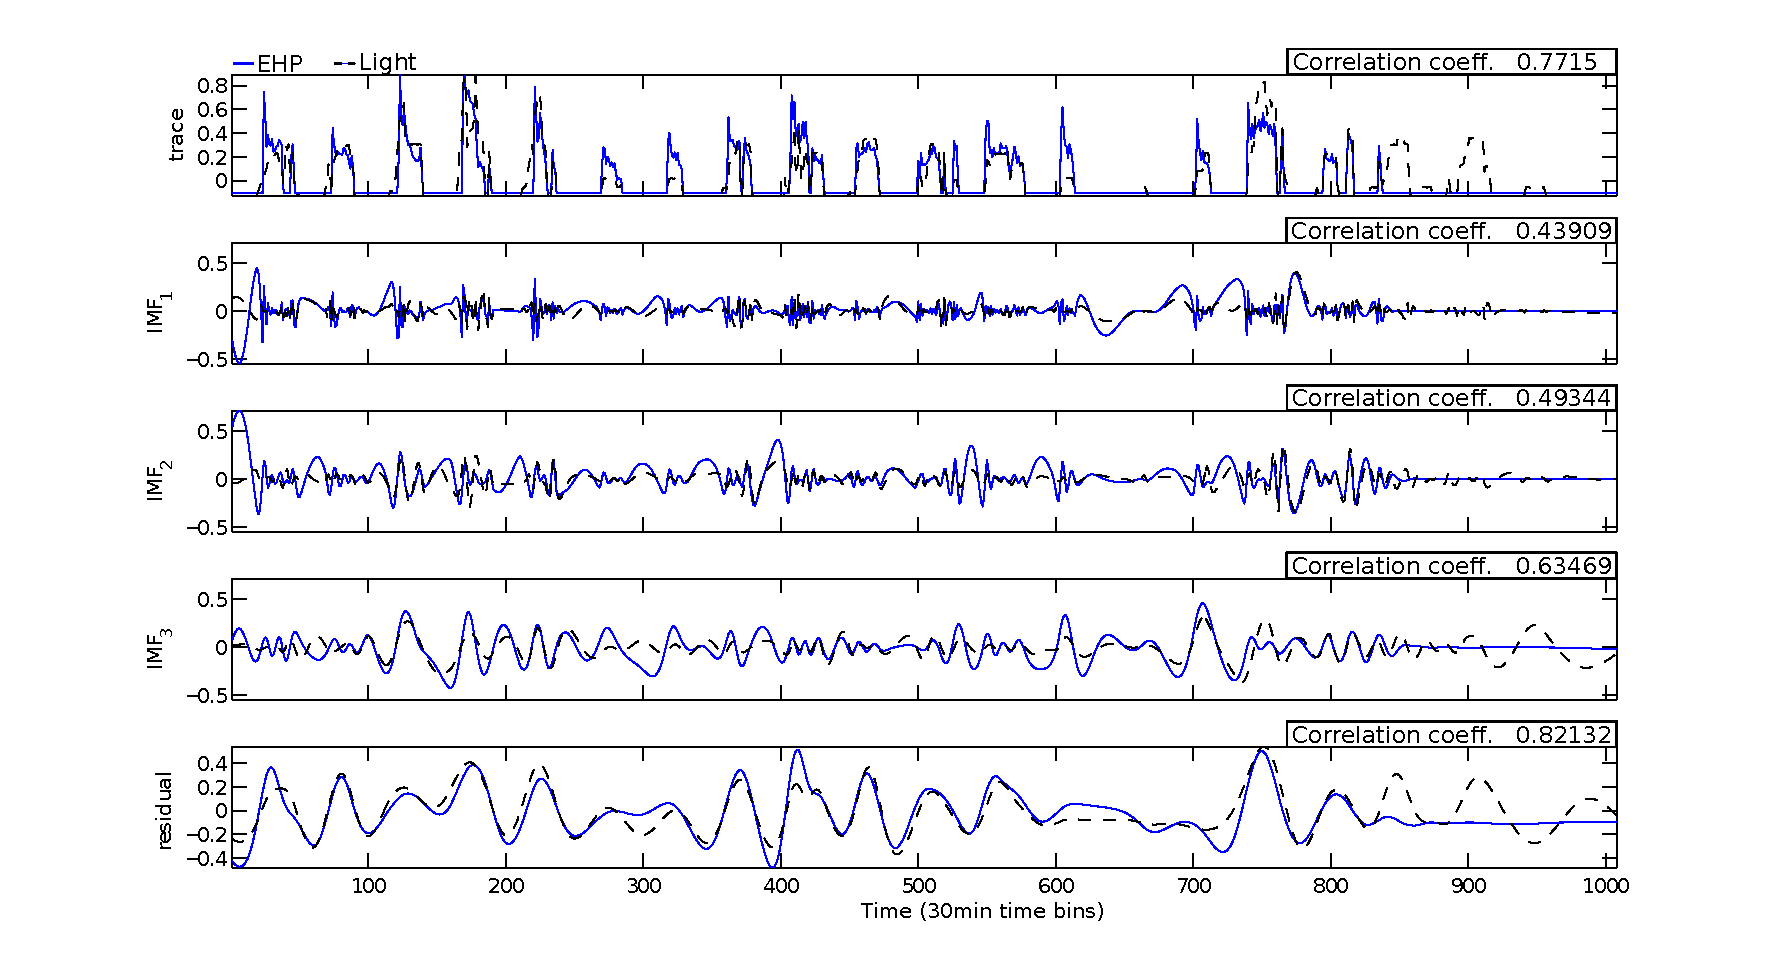
\includegraphics[width=1.2\textwidth]{figs/emd_25_26-eps-converted-to}
\vspace{-1cm}
\caption{Decomposition of the EHP and light trace using bivariate EMD. IMFs correlation coefficients highlight the intrinsic relationship of the two traces.}
\label{fig:emd}
\end{figure*}

% The intent of the Green University of Tokyo Project (GUTP) \cite{gutp} is to reduce the university environmental impacts associated to its electric energy consumption.
% The first step of this project was to deploy sensors at the Building No.2 of the Faculty of Engineering 
% Electric power consumption of a 12 floors building containing researchers office and classroom.
% 1215 sensors monitoring different devices...

%received attention in the past \cite{ogawa:lncs2011}.

For this investigation, we focus on a three-week span in the summer of 2011 (from July 4th to July 24th).
The dataset captures regular work days, weekends, and one holiday (July 18th).  This timeframe captures
the typical usage of the equipment, triggered by occupant activity.  For the initial
analysis, we focus on three sensors; two water pumps and a light feed.  The first pump is an 
``electric heat pump'' and is labled as EHP, the second  is a ``gas heat pump''
and labeled as GHP.  The room lighting system serves the same room as the EHP.  The GHP
serves a different room on the same floor.  The expanded portion of our analysis pivots around the EHP
and does a pairwise comparison between it and all other sensors in the building.
Computationally, this approach does not scale to a large number of sensors.  For future work, we will
examine various heuristics to narrow the search space before running pairwise comparisons.

% includes one day holiday (July 18th)
% 3 different sensors:
% \begin{itemize}
%  \item Two are measuring the electric power consumption of two devices from the same room; an electric heat 
%  		pump (EHP) and the room lighting system.
%  \item One is measuring the electric power consumption of a gas heat pump (GHP) that is pumping water to cool 
%  		a different room in the same building.
% \end{itemize}

% Later we expand our analysis to include all the sensors in the building.


\section{Problem statement and Initial approach}\label{problem}
% In our analysis, we are focused on finding devices that are correlated in their use over time.  Therefore, the
% main objective is to examine how device traces relate to one another.  The wish to identify
% correlated device-trace patterns at large spatio-temporal scales.

In buildings, metadata is poorly and unsystematically managed within a single system domain.  Moreover, 
with the ever growing number of additional sub-meters, it is important to quickly integrate
sensor data from multiple systems to understand the full state of the building.  It is also important to 
understand how sensors are used in concert.  Anomalies in usage may indicate underlying problems with 
the equipment or inefficient/incorrect usage.  

Figure \ref{fig:raw} shows the raw traces for the three devices discussed in 
the previous section (EHP, GHP, light). All three exhibit a diurnal usage pattern.  On weekends, each
draw less power.   For our initial analysis, we calculated the pairwise 
correlation coefficient for all sensors in the set.  The correlation coefficient for 
 the EHP and light is $0.7715$ and the correlation coefficient for the EHP and GHP is $0.6370$.
Running correlation across them yields high correlation coefficients, mostly
due to their underlying daily usage pattern.


% \begin{figure}[t!]
% \centering
%  \subfigure[EHP trace]{\label{fig:raw_ehp}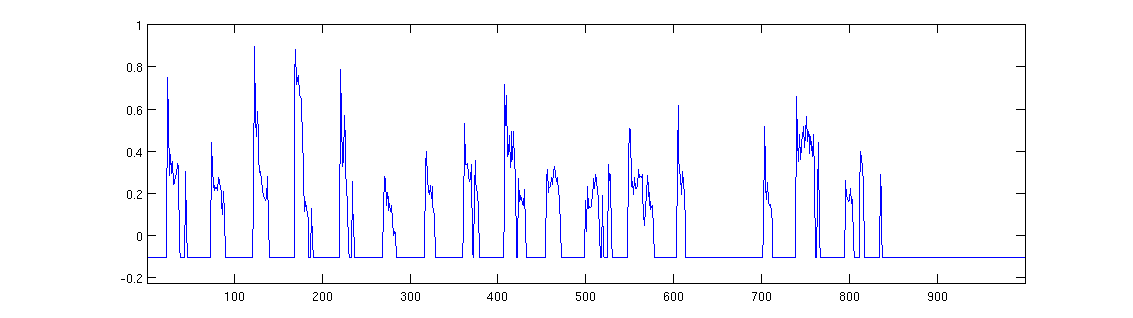
\includegraphics[width=.4\textwidth]{img/25.png}}
%  \subfigure[Light trace]{\label{fig:raw_light}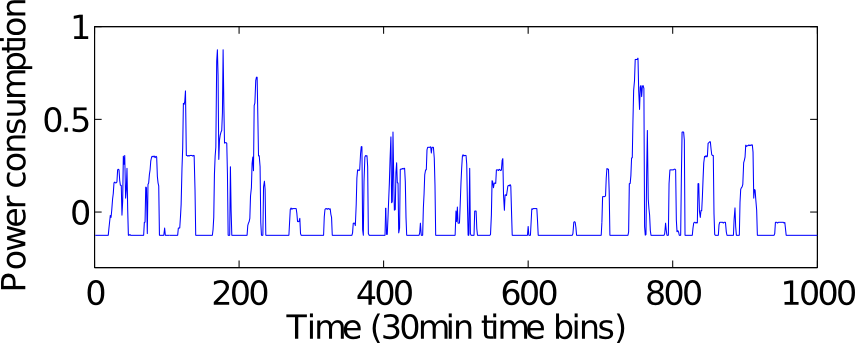
\includegraphics[width=.4\textwidth]{img/26.png}}
%  \subfigure[GHP trace]{\label{fig:raw_ghp}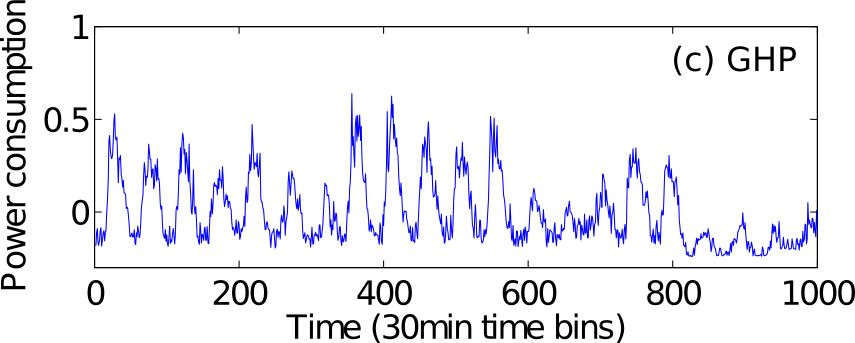
\includegraphics[width=.4\textwidth]{img/41.png}}
%  \caption{Traces from three different sensors captured in 2011 from July 4th to July 24th. Data is normalized and aggregated into 30 minutes time bins.}
%  \label{fig:raw}
% \end{figure}


Our initial results were not surprising.  The diurnal pattern dominates the comparison between the sensors.
Weather is the main driver for this behavior and it affects the readings in almost all of the
sensors in our dataset.  Cross-correlation on raw sensor data is insufficient for filtering intrinsically related
behavior.  Upon closer examination of the data we assess the following:

\begin{itemize}
\item The main underlying diurnal trend occurs in almost all the traces.
\item Occupancy and room activities occur at random times during the day and change 
		at a higher frequency than weather patterns.
\item Sensors that serve the same location observe the same activities.  Therefore, their underlying
		measurements should be correlated.
\end{itemize}

In order to uncover these relationships we must remove low-frequency trends in the traces and
compare the readings at high frequencies.

% \begin{table}
% \begin{center}
% \begin{tabular}{|l|l|l|l|l|l|}
% \hline
% × & Raw trace & 1st IMF & 2nd IMF & 3rd IMF & Residual\\ \hline
% EHP, Light & 0.7715 & 0.43909 & 0.49344 & 0.63469 & 0.82132 \\ \hline
% EHP, GHP & 0.6370 & 0.0060274 & 0.063546 & 0.16764 & 0.79378 \\ \hline
% \end{tabular}
% \caption{Correlation coefficients of the analyzed trace and their IMFs uncovered by EMD}
% \label{tab:corr}
% \end{center}
% \end{table}
% \subsection{Simple Scenario}

\begin{figure*}[tb]
\hspace{-2cm}
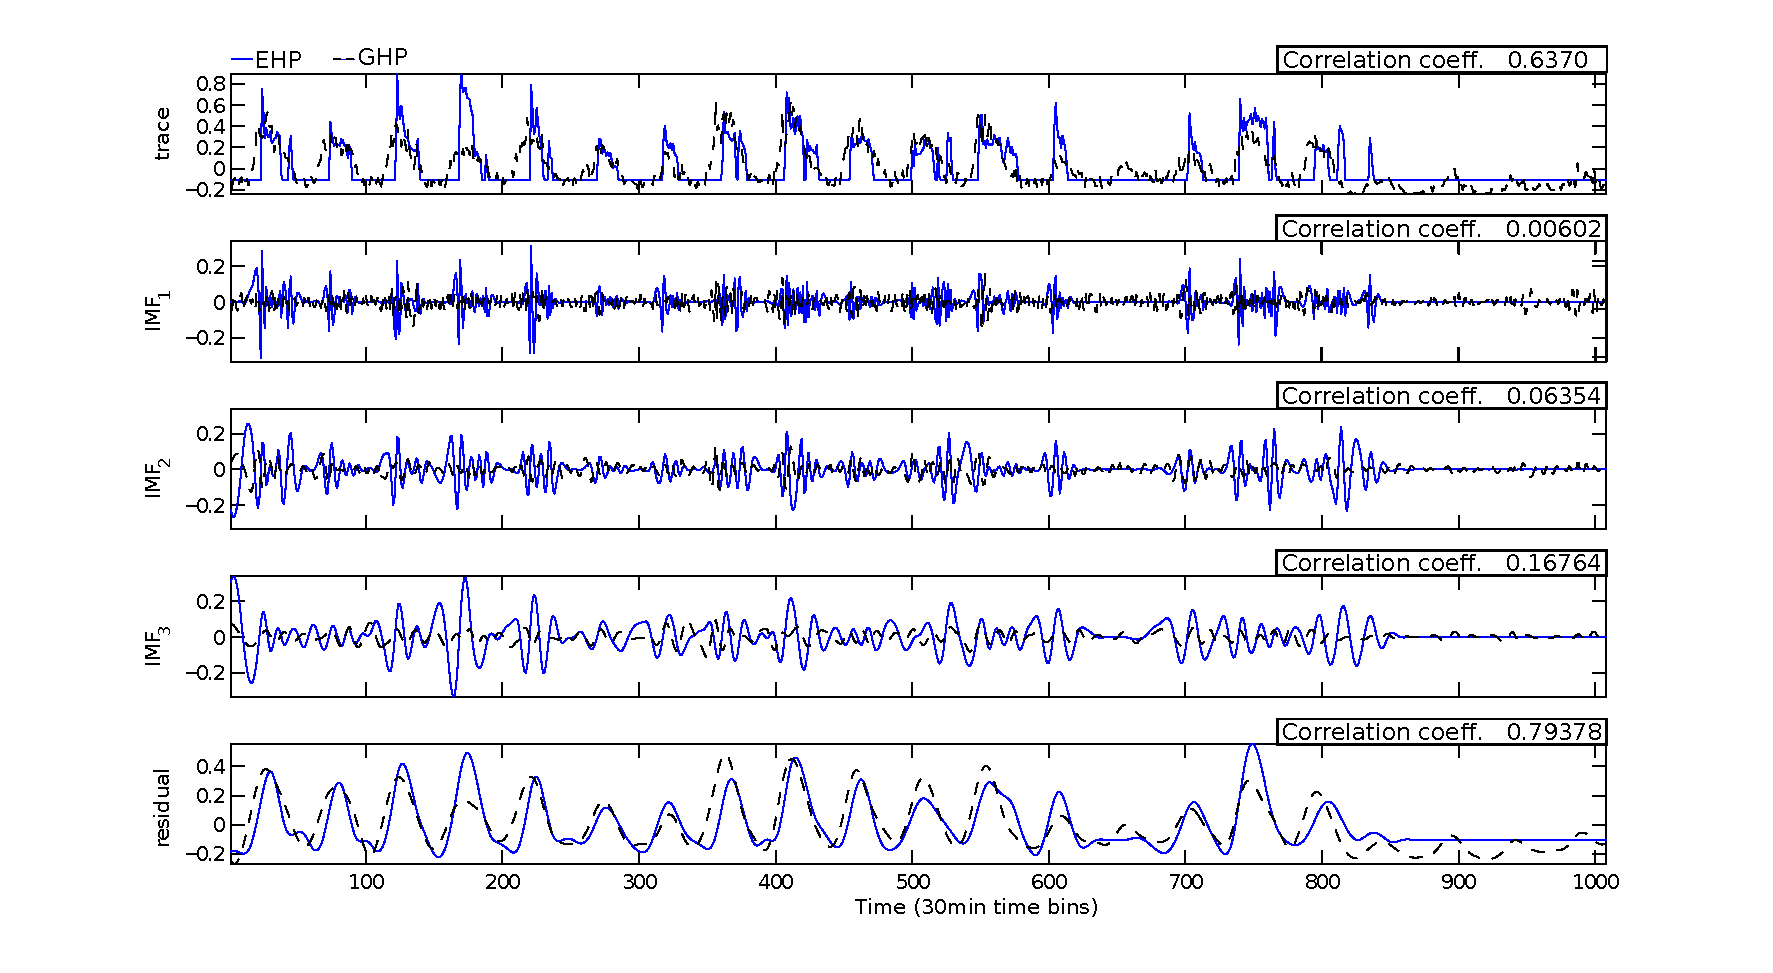
\includegraphics[width=1.2\textwidth]{figs/emd_25_41-eps-converted-to}
\vspace{-1cm}
\caption{Decomposition of the EHP and GHP trace using bivariate EMD. IMFs correlation coefficients highlight the intrinsic independence of the two traces.}
\label{fig:emd2}
\end{figure*}

% The small difference between the two computed correlation coefficients is misleading as one could conclude that the three signals are correlated and the corresponding devices are activated by a single action.

% The high correlation coefficients obtained for these three signals result .... weekly pattern....
% small difference = local fluctuation...

% this high score comes from the fact that the two devices are monitoring offices that are weekly used.

% Indeed the weekly pattern of the data trump the correlation coefficients....

% How to inspect only the local fluctuations...?
% we'd like to have an elegant solution (i.e. not specifying the interesting time scale)

